\chapter{Architettura MVC}
L'architettura MVC, per la prima volta presentata nel 1988 da Glenn E. Krasner e Stephen T. Pope nel loro articolo “A Cookbook for Using the Model-View-Controller User Interface Paradigm in Smalltalk-80", rappresenta un caposaldo della programmazione e una delle architetture più utilizzate sia lato front-end che back-end.

L'elemento base su cui si fonda MVC è la modularità del codice e la portabilità dei vari componenti che formano l'applicazione. Per ottenere ciò si è teorizzato di dividere quest'ultima in tre parti ben distinte: le parti che ne rappresentano la struttura astratta, il modo in cui queste vengono presentate e il modo con cui l'utente ci interagisce. Questa divisione permette l'isolamento delle unità funzionali dell'applicazione in modo da facilitarne il debugging e la scalabilità, oltre al fatto di migliorare la riusabilità dei componenti creati seguendo questo pattern \cite{KrasnerAndPopeOnMVC}.

\section{Divisione dei compiti}
La divisione dei compiti nell'architettura MVC, come è stato detto precedentemente, avviene attraverso Model, View e Controller. Questi tre elementi fondamentali dell'applicazione sono interconnessi e ognuno ha un compito specifico, isolato dagli altri, a cui deve attenersi.

\begin{wrapfigure}{r}{7cm}
\centering 
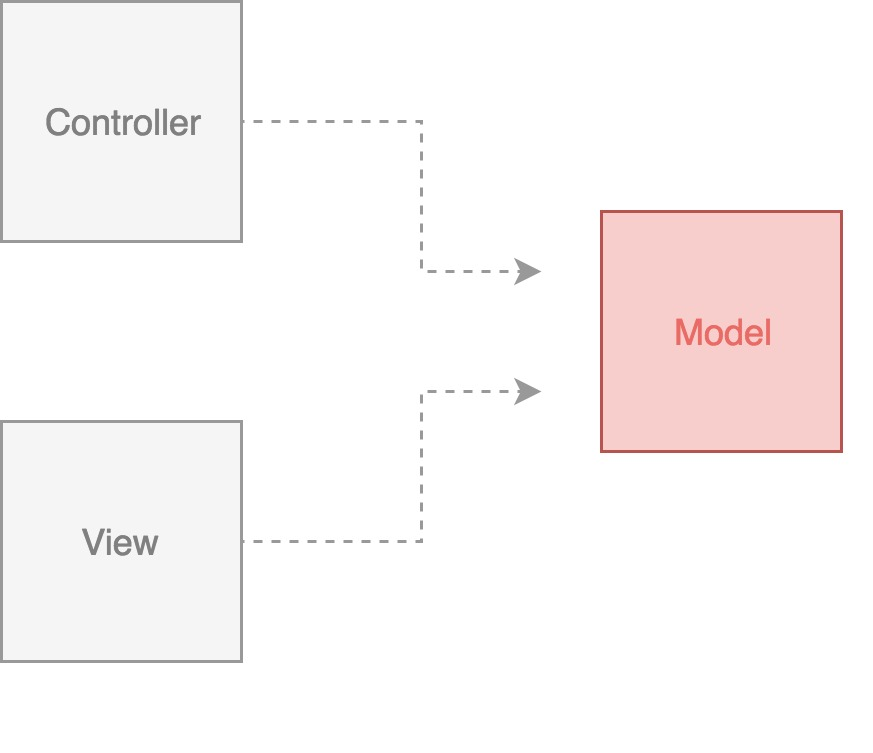
\includegraphics[width=5.5cm]{./images/MVCdefault}
\caption{Architettura MVC classica.}
\end{wrapfigure}

Il Model rappresenta i dati che formano tutta o una parte dello stato dell'applicazione e come essi mutano. E' possibile immaginare questo componente come un oggetto che identifica un elemento specifico del servizio e ne descrive come il suo stato muta ad una eventuale azione. Il Model è “cieco", nel senso che tutto ciò che fa è mantenere dati e descrivere come essi mutano non avendo in alcun modo né la possibilità di conoscere in che modo influenzano l'applicazione né la capacità autonoma di effettuare modifiche su di essi se non sotto specifica istruzione del Controller.

I componenti che compongono la View hanno l'obiettivo di rappresentare i dati del Model in una forma facilmente comprensibile all'utente finale. Nell'architettura standard MVC il ruolo della View era piuttosto dinamico e organizzava i suoi aggiornamenti discutendo direttamente con il Model ed ottenendo i dati da esso, lasciando al Controller il compito di gestire gli input dell'utente. In questo modo l'architettura era organizzata con il Model come componente centrale togliendo importanza al Controller.

\noindent
Andando avanti nel tempo e con la comparsa di sempre più framework ispirati a questo pattern, l'evoluzione ha cambiato leggermente le regole standard dettando che la View dovrebbe avere il meno possibile un ruolo “attivo" di lettura degli aggiornamenti del Model, e che la gran parte delle informazioni dovrebbe passare attraverso il Controller che diventa così l'elemento principale addetto alla logica \cite{HopkinsOnMVCandPHP}.

\begin{wrapfigure}{l}{7cm}
\centering 
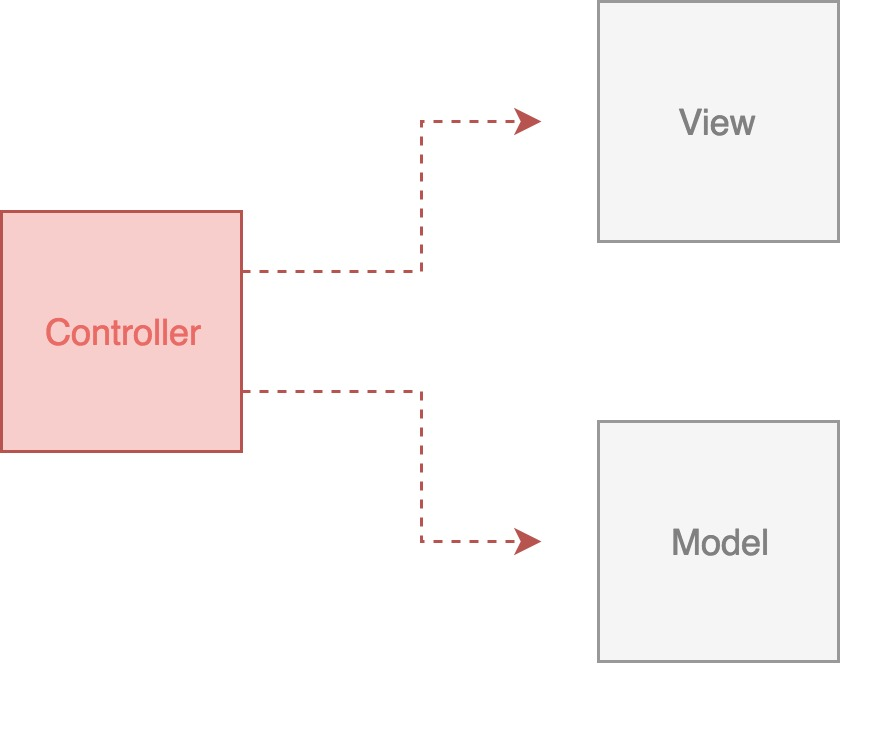
\includegraphics[width=5.5cm]{./images/MVCpassiveview}
\caption{Architettura MVC recente.}
\end{wrapfigure}

Il Controller, nella versione classica dell'architettura MVC, si occupa solo ed esclusivamente di gestire gli input forniti dall'utente, trasmettendo le informazioni ricevute al Model. E' bene tenere presente che ogni Controller viene eseguito solamente a seguito di una azione che l'utente ha intrapreso dalla View e che quest'ultima ha un collegamento diretto con il Model comunicando attraverso il pattern Observer per adeguarsi ai vari cambiamenti dello stato.
Nelle versioni più recenti dell'architettura MVC invece, il Controller assume sempre di più la parte centrale incaricata di organizzare e collegare le altre due. Non solo si occupa di gestire i vari eventi ed input generati dall'utente, ma si occupa anche di fornire e filtrare i dati del Model alla View, sottolineando la loro natura in questo caso più statica.

\section{MVC nel front-end}
L'architettura MVC è nata per risolvere il problema dell'organizzazione e della struttura del codice in applicazioni desktop scritte in Smalltalk-80. La sua versatilità e potenza ha tuttavia fatto si che anche tutt'ora questo paradigma venga utilizzato nella stragrande maggioranza delle applicazioni, specialmente lato back-end.
Con la nascita delle SPA e con lo spostamento della logica sempre più verso il front-end tuttavia si sono presentati diversi problemi con l'architettura MVC classica i quali hanno spinto quest'ultima a modificarsi ed adattarsi al nuovo ambiente.

Lato front-end l'architettura MVC assume diverse forme a seconda del tipo di caratteristiche di cui abbiamo bisogno. Molti framework in Javascript tentano di includere il lavoro del Controller all'interno della View, altri al contrario rendono quest'ultima completamente passiva spostando tutta la logica al Controller,  aggiungono semplicemente nuovi livelli di divisione. Queste differenti architetture derivate vengono associate ad una macro-categoria chiamata \textit{MV*} (l'asterisco al posto della “C" di Controller sta a significare che questo è l'elemento che viene solitamente sostituito o modificato) dalla quale è possibile estrapolare due tra i più famosi ed utilizzati paradigmi lato front-end: MVP e MVVM \cite{OsmaniOnJSFrameworks}.

\subsection{MVP}
L'architettura MVP nasceva nel 1990 nell'azienda Talingent e veniva utilizzata per lo sviluppo di applicazioni in C++ e Java \cite{Potel1996mvp}. E' stato successivamente ripresa da vari framework Javascript tra cui uno dei più famosi è sicuramente Backbone.js.
Mentre nella versione classica di MVC, la View osservava il Model e si modificava di conseguenza, l'evoluzione di questo pattern ha fatto si che il ruolo di osservatore passasse sempre più al Controller, ora chiamato Presenter, che costituisce un vero e proprio elemento centrale ed intermediario, eliminando quindi completamente la logica dalla View.

\begin{figure}[h]
\centering 
\vspace*{0.5cm}
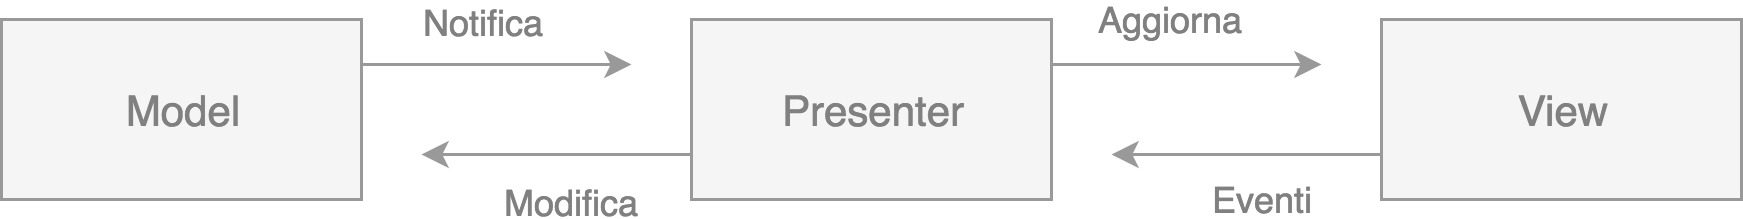
\includegraphics[width=13cm]{./images/MVPworkflow}
\caption{Architettura MVP.}
\vspace*{0.5cm} 
\end{figure}

\noindent
MVP è un paradigma utilizzato specialmente per applicazioni a livello enterprise, con View complesse e grandi quantità di interazioni da parte dell'utente in quanto tutta la logica risiede nel Presenter rendendo l'applicazione semplice da testare e staccando la View dal resto rendendola particolarmente riutilizzabile all'interno del codice.
Tuttavia le differenze tra le architetture MVC e MVP sono solo a livello semantico, interpretando cioè diversamente un componente comune ad entrambe. Molti problemi più radicati che troviamo nella prima quindi si vengono comunque a presentare nella seconda \cite{OsmaniOnJSFrameworks}.

\subsection{MVVM}
L'architettura MVVM è stata per prima definita da Microsoft in un post del 2005 di John Grossman \cite{GossmanOnMVVM}. E' nata come una architettura per la creazione di applicazioni con Windows Presentation Foundation (WPF) ed è stata successivamente implementata con un discreto successo in framework Javascript come Knockout.js.

Questo paradigma si basa completamente sulla sincronizzazione della View attraverso il pattern Observer. La logica dell'applicazione quindi questa volta è posizionata quasi interamente nella View e, mentre il Model si comporta come da norma solamente da “memoria", questa ne osserva i cambiamenti e si aggiorna di conseguenza. La vera differenza è che in questo caso le azioni dell'utente sono gestite direttamente dalla View, in quanto il vincolo posto sui dati è bidirezionale (modificando l'elemento in input nella View viene automaticamente modificato il valore referenziato).
La View tuttavia non può leggere direttamente i dati di cui ha bisogno dal Model, i quali nella maggior parte dei casi sono grezzi e hanno bisogno di essere filtrati e lavorati. Per questo è stato creato un nuovo componente, che sostituisce il Controller, chiamato ViewModel il quale si pone come livello passivo intermedio tra Model e View, ed estrapola i dati utili dal primo e li rende disponibili in maniera comprensibile al secondo, oltre anche a fornire funzioni utili alla gestione dello stato e degli eventi \cite{OsmaniOnJSFrameworks}.

\begin{figure}[h]
\centering 
\vspace*{0.5cm}

\includegraphics[width=13cm]{./images/MVVMworkflow}
\caption{Architettura MVVM.}
\vspace*{0.5cm} 
\end{figure}

\noindent
Uno dei punti forti dell'architettura MVVM implementata dai più recenti framework Javascript riguarda l'astrazione della View per l'utilizzo dei vincoli di dati bidirezionali (Two-ways Data Bindings) del ViewModel direttamente all'interno del DOM.

\begin{listing}[ht]
\inputminted{jsx}{sources/exampleMVVMDataBinding.js}
\caption{Esempio di vincolo di dati nel DOM.}
\label{exampleMVVMDataBinding}
\end{listing}

\noindent
Da una parte questi facilitano enormemente l'implementazione dell'interfaccia e consentono di ridurre in maniera considerevole la logica da implementare a parte all'interno del ViewModel, dall'altra sono considerati un tipo di programmazione obsoleta che mischia la logica con il linguaggio di markup.

\section{MVC e il flusso dei dati}